
\newcommand{\meff}{m_\mathrm{eff}}
\newcommand{\meffs}{m_\mathrm{eff}^2}

\newcommand{\bk}{\mathbf{k}}
\newcommand{\bkp}{\mathbf{k}^\prime}
\newcommand{\by}{\mathbf{y}}
\newcommand{\bff}{\mathbf{f}}

\newcommand{\ket}[1]{\left|#1\right\rangle}
\newcommand{\bra}[1]{\left\langle#1\right|}
\newcommand{\braket}[2]{\left\langle#1\middle|#2\right\rangle}
\newcommand{\bracket}[3]{\left\langle#1\middle|#2\middle|#3\right\rangle}


\chapter{The Runge-Kutta-Wentzel-Kramers-Brillioun method}
\label{chap:RK}

\section{Introduction}
\label{sec:introduction}
The numerical solution of linear, ordinary differential equations is of critical importance throughout science and mathematics. In this letter we suggest an efficient approach for navigating highly oscillatory numerical solutions.

Most traditional numerical solvers of differential equations use a generalisation of Runge-Kutta (RK) techniques~\citep{Press+2007}. These apply Taylor's theorem to create a stepping scheme whereby the value of the solution is updated using derivative information. Good solvers will also incorporate adaptive step-size control.
Whilst RK techniques are an excellent workhorse for solving a wide variety of problems, they are known to struggle to solve equations with highly oscillatory solutions.

On the other hand, the Wentzel-Kramers-Brillouin (WKB) method is a well established analytical approach for approximately describing oscillatory solutions~\citep{RHB,Bender+2010}. Historically this has been used to approximate the global shape and characteristics of an oscillating solution with a ``slowly changing'' frequency.

We propose that one may combine the two approaches to create a reliable general tool for the numerical solution of oscillatory differential equations, and term the result RKWKB\footnote{Readers with experience in the field will note that, as Cambridge authors, we should be insisting on an additional `J' in WKB (for Jeffreys). Given the length of our proposed acronym, we have opted to use the more efficient nomenclature.}.

We note that this approach is similar to the work of \cite{Iserles02globalerror,Iserles01thinkglobally}, and explore the similarities and differences in Section~\ref{sec:iserles_comparison}.


\section{Background}
\subsection{Oscillating solutions}
We seek to create a numerical method which efficiently solves linear differential equations such as:
\begin{equation}
  \ddot{x}(t) + {\omega(t)}^2x(t) = 0,\qquad \omega(t)\in\mathbb{R}.
  \label{eqn:lode}
\end{equation}
If $\omega(t)=\omega = \mathrm{constant}$, then the solutions are sinusoidal: $x\propto \exp{(\pm i \omega t)}$. If $\omega(t)$ changes slowly with $t$, then the solutions are approximately sinusoidal with a slowly varying frequency and amplitude (these ideas will be made more concrete in Section~\ref{sec:wkb}). An example of such a solution can be seen in Figure~\ref{fig:airy}.

In general, any second order linear differential equation may be transformed into the form of~(\ref{eqn:lode}) by either changing the independent variable $t$ or dependent variable $x$. The method we shall describe can easily be adapted to other linear differential equations, but we shall work with~(\ref{eqn:lode}) for its simplicity of exposition.

Equation~(\ref{eqn:lode}) is ubiquitous in physics, particularly in quantum mechanics. The authors' particular interest in its efficient solution comes from work in quantum fields in curved spacetime.



Over the next two subsections we will review the traditional techniques available for solving equations such as~(\ref{eqn:lode}).

\begin{figure}[]
  \centering
  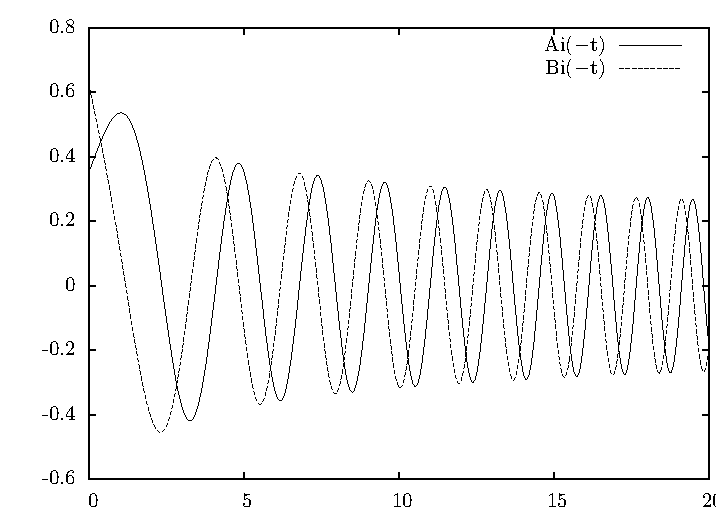
\includegraphics[width=\textwidth]{airy}
  \caption{The real and imaginary parts of the function $\mathrm{Ai}(-t) + \mathrm{Bi(-t)} i$, where $\mathrm{Ai}$ and $\mathrm{Bi}$ are the Airy functions of the first and second kind. This is a solution to the equation ${\ddot{x}(t) + t x(t) = 0}$ (equation~\ref{eqn:airy_equation}).\label{fig:airy}}
\end{figure}


\subsection{Runge-Kutta theory}
\label{sec:rk}
We briefly review the theory of numerically solving ordinary differential equations, before discussing why Runge Kutta techniques are an inefficient tool for solving equations such as~(\ref{eqn:lode}).
For a more detailed introduction to the numerical solution of ordinary differential equations we recommend~\cite{Press+2007}.

A general non-linear differential equation in $n$ variables can be written in terms of vectors as:
\begin{equation}
  \dot{\by}(t) = \bff(\by(t),t).
  \label{eqn:ode}
\end{equation}
Note that any higher order differential equation can be re-written in this form by introducing new variables for each of the higher derivative terms.

Runge-Kutta methods work effectively by generalising the Taylor expansion:
\begin{equation}
  \by(t+h)  = \by(t) + h\:\bff(\by(t),t) + \mathcal{O}(h^2).
  \label{eqn:euler}
\end{equation}
Given the value of a solution $\by_j$ at some time $t_j$, one may advance to the value of the solution $\by_{j+1}$ at some finite time later $t_{j+1} = t_j + h$ by using the recursion relation:
\begin{align}
  \by_{j+1} &=  \by_{j} + h\:\bff(\by_j,t_j),
  \label{eqn:y_step}\\
  t_{j+1} &=  t_{j} + h.
  \label{eqn:t_step}
\end{align}
This is termed {\em Euler's method}, and for arbitrarily small $h$ will recover the solution to any desired accuracy. It is termed {\em first order\/} since each step is accurate to $\sim \mathcal{O}(h)$.

Euler's method is normally impractical for real numerical work. Runge-Kutta schemes work by generalising~(\ref{eqn:euler})~\&~(\ref{eqn:y_step}) by including additional intermediate function evaluations that integrate~(\ref{eqn:ode}) with greater accuracy.

A possibly more important adjustment is to equip the algorithm with the ability to choose the step size $h$ according to the accuracy required. A popular stratagem is to run two steps, one of order $p$, and another of order $p-1$, and use the difference between the two as an estimate of the error. Particularly smart algorithms use the same function evaluations for both orders. An example of this is the Runge-Kutta-Fehlberg $4(5)$ method detailed in Section~\ref{sec:rkf}.

All methods based on this principle struggle to solve equations such as~(\ref{eqn:lode}) when the algorithm must scale a very large number of peaks and troughs. Errors accumulate rapidly in these approaches, even if the variation of $\omega(t)$ in $t$ is very simple. Given the regularity of the solution from Figure~\ref{fig:airy}, one would imagine that there should be a more efficient method.


\subsection{WKB theory}
\label{sec:wkb}
WKB approaches are designed to solve linear ordinary differential equations like~(\ref{eqn:lode}) in the limit of a ``slowly varying'' $\omega(t)$: i.e.\ the fractional change in frequency $\frac{\Delta\omega}{\omega}$ over several time periods $\Delta t \sim \frac{2\pi}{\omega}$ is relatively small.
A systematic way of phrasing this is to rescale the independent variable of~(\ref{eqn:lode}) so $t\rightarrow T t$:
\begin{equation}
  \ddot{x}(t) + T^2{\omega(t)}^2x(t) = 0,\qquad \omega(t)\in\mathbb{R}.
  \label{eqn:lode_T}
\end{equation}
If $T\gg1$ then $\omega$ is slowly varying, or equivalently the solutions have very rapid oscillations (large $\omega$). Given this, one can expand the solutions in terms of complex exponential functions:
\begin{equation}
  x(t)\sim \exp\left( \frac{1}{T}\sum\limits_{n=0}^{\infty} S_n(t)\: T^n \right).
  \label{eqn:asymp}
\end{equation}
Substituting this into~(\ref{eqn:lode_T}) and setting each coefficient of $T$ equal to zero yields a sequence of solvable equations. One finds the first four solutions are:
\begin{align}
  S_0(t) &= \pm i \int^t \omega(\tau)\: d\tau,
  \label{eqn:S0}\\
  S_1(t) &= -\frac{1}{2}\log \omega(t),\\
  S_2(t) &=  i \int^t \frac{1}{4}\frac{\ddot{\omega}(\tau)}{\omega^{2}(\tau)} - \frac{3}{8}\frac{\dot{\omega}^2(\tau)}{\omega^{3}(\tau)}\: d\tau, \\
  S_3(t) &=  \frac{1}{8}\frac{\ddot{\omega}(t)}{\omega^{3}(t)} - \frac{3}{16} \frac{\dot{\omega}^{2}(t)}{\omega^{4}(t)}.
\end{align}
Note that at $0$\textsuperscript{th} order, the solution is $x\propto\exp\left( \int \omega dt \right)$, which should be compared with the traditional sinusoidal solution.
Typically $T$ is considered a power counting parameter, and set equal to $1$ at the end of the analysis.

There are two integration constants associated with the either sign of equation~(\ref{eqn:S0}). The other integration constants from the remaining equations may be absorbed into the first two. The $n$\textsuperscript{th} order solution thus takes the form:
\begin{align}
  x_\mathrm{WKB}^{(n)}[A_{\pm}](t) =&
  \left( A_{+} e^{S_0(t)} + A_{-} e^{-S_0(t)} \right)
  \nonumber\\
  &\times \exp\left( \sum_{i=1}^n S_i(t) \right).
  \label{eqn:solution}
\end{align}
If one has initial conditions at time $t_0$:
\begin{equation}
  x(t_0) = x_0, \qquad \dot{x}(t_0)=\dot{x}_0,
  \label{eqn:i_c}
\end{equation}
then the coeffients $A_\mu$ may be determined by:
\begin{align}
  A_\pm^{(n)}(x_0,\dot{x}_0,t_0) =& \frac{1}{2}\exp{\left( \mp S_0(t_0) - \sum_{i=1}^n S_i(t_0) \right)}
  \nonumber\\
  &\times\left( x_0 \pm  \frac{\dot{x}_0-x_0\sum_{i=1}^n \dot{S}_i(t_0)}{\dot{S}_0(t_0)}\right).
  \label{eqn:i_c_Apm}
\end{align}
For further detail on the intricacies of WKB approaches, the reader should consult \cite{RHB,Bender+2010}.

\section{The RKWKB method}
Our strategy is to combine the versatility of RK methods with the power of WKB in dealing with oscillating solutions. We term the combination RKWKB.

Given a function $\omega(t)$, one proposes a step in time of $h$ to be accompanied by an updating of the solution $x_j$ via:
\begin{align}
  x_{j+1} &= x_\mathrm{WKB}^{(n)}[A_\pm(x_j,\dot{x}_j,t_j)](t_j+h),
  \label{eqn:WKB_x_step} \\
  t_j &= t_j+h,
  \label{eqn:WKB_t_step}
\end{align}
where $x_\mathrm{WKB}^{(n)}[A_{\pm}]$ is given by~(\ref{eqn:solution}) and $A_{\pm}$ is given by~(\ref{eqn:i_c_Apm}).
To paraphrase the above, one matches the $n$\textsuperscript{th} order WKB solution onto the current values of $x_j$ and $\dot{x}_j$, and uses this to extrapolate the solution by a time step of $h$. Since WKB naturally encodes the oscillatory nature of the solution, this will allow step sizes $h$ to be far larger than a single period of oscillation. 

\subsection{Step size adjustment}
To tune the step size $h$, we use the same strategy as adaptive Runge-Kutta schemes. We compute both the order $n$ and order $n-1$ WKB solutions, and use the fractional difference between the two:
\begin{equation}
  \varepsilon = \left|\frac{x^{(n)}-x^{(n-1)}}{x^{(n)}}\right|,
  \nonumber
\end{equation}
as an estimate of the truncation error. 

We now assume that the desired accuracy is $\alpha$. If $\varepsilon<\alpha$ then the solution is within the desired tolerance, and the algorithm makes a step of size $h$. $h$ is then increased for the next iteration. If $\varepsilon>\alpha$ then the step is unsuccessful, and the step size is reduced. $h$ may therefore be efficiently updated between attempts via:
\begin{equation}
  h \to h\times\left\{
  \begin{array}{lr}
    (\alpha/\varepsilon)^{1/n} &: \varepsilon<\alpha \\
    (\alpha/\varepsilon)^{1/(n-1)} &: \varepsilon>\alpha. \\
  \end{array}
  \right.
  \label{eqn:h_update}
\end{equation}
This allows the step size to increase in the regions where the initial step size is unnecessarily small, whilst ensuring that the step size is always small enough to keep forecasts within a given error margin.

\subsection{Dynamic switching}
In general, one cannot expect the WKB expansion to be efficient throughout the solution region. If $\omega$ is too small, or too quickly varying, then the step size $h$ will decrease to an inefficiently small size. This problem can be countered by simultaneously attempting a step using a standard adaptive RK method. One chooses between RK and WKB by selecting the method with the smallest error. This provides a natural switching mechanism, without having to delve into the details of whether WKB is valid or not.

We choose the Runge-Kutta-Fehlberg $4(5)$ method for our alternative solver, which is detailed in Section~\ref{sec:rkf}. However, this may be substituted with any ODE solver according to the users preference.

\section{Example: The Airy equation}


As an example of the RKWKB approach, we apply it to the Airy equation:
\begin{align}
  0=\ddot{x}(t) &+ t\: x(t) ,
  \label{eqn:airy_equation}\\
  x(0)=\frac{3^{-2/3}+3^{-1/6}i}{\Gamma(2/3)},
  &\qquad
  \dot{x}(0) = \frac{3^{-1/3}-3^{1/6}i}{\Gamma(1/3)},
  \nonumber\\
  \Rightarrow x(t) = \mathrm{Ai}(-t) &+ \mathrm{Bi}(-t)\:i,
  \label{eqn:airy_solution}
\end{align}
whose solution is depicted in Figure~\ref{fig:airy}. This is often quoted as being a ``maximally hard'' problem for RK machinery to solve, since the frequency steadily increases, causing the step size to get smaller as the algorithm goes deeper into the solution.

We set the desired relative error to be $10^{-4}$. The algorithm remains in the RK regime until $t\sim5$. When the WKB solver is activated, instead of following every oscillation of the solution, it rapidly speeds up, skipping many oscillations. This is detailed in Figure~\ref{fig:data}.

The error compared to the true solution is detailed in Figure~\ref{fig:error}. Here we find that initially the error is small, but grows$\sim\mathcal{O}(h^{2s} t^{s+5/4})$ where $s=4$ is the order of the RK method~\citep{Iserles02globalerror}. After the WKB regime is entered, it begins to make huge strides, and the error levels off.

In contrast to a ``pure'' RK method, the RKWKB method finds the Airy equation maximally {\em easy}.



\begin{figure}[]
  \centering
  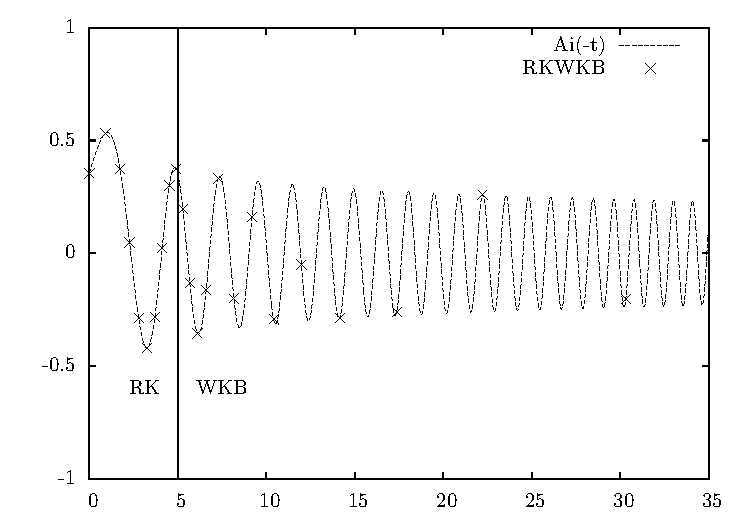
\includegraphics[width=\textwidth]{data}
  \caption{The RKWKB method compared with the analytical solution. The algorithm starts at $t=0$ in the RK regime, since $\omega$ is varying quickly relative to the oscillation period. At $t=5$ it becomes more efficient to use the WKB regime, and the points start to increase in separation. By $t=15$ the algorithm is skipping multiple periods, and the step size $h$ increases exponentially.\label{fig:data}}
\end{figure}

\begin{figure}[]
  \centering
  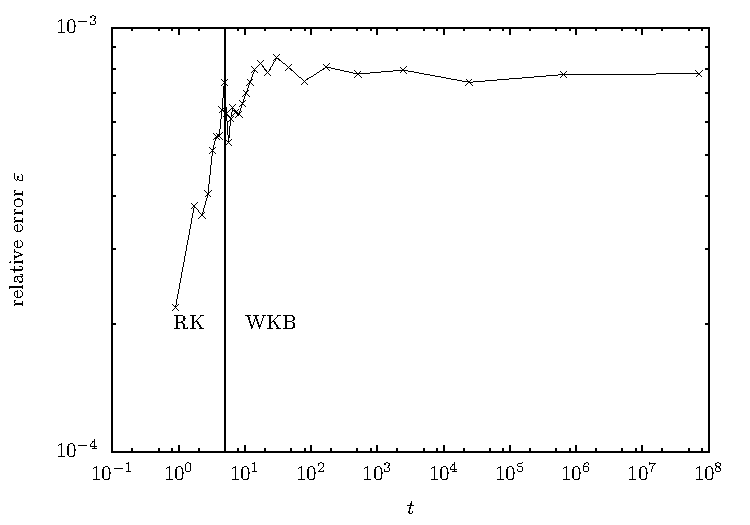
\includegraphics[width=\textwidth]{error}
  \caption{Fractional difference between the analytical solution and RKWKB solution from Figure~\protect\ref{fig:data}. The algorithm's fractional error begins at $t=0$ with an error of $\sim10^{-4}$, but rises in the RK phase. This is to be expected as RK methods accumulate errors (particularly for oscillatory solutions). Upon entering the WKB region, the fractional error levels off. Note the rapidly increasing step size, and accuracy at extremely late times $t$. To the authors' knowledge, no numerical scheme to date has demonstrated the ability to solve the Airy equation~(\protect\ref{eqn:airy_equation}) to times as late as this.\label{fig:error}}
\end{figure}




\section{Comparison with the Iserles approach}
\label{sec:iserles_comparison}
Iserles has written extensively on the difficulty of solving problems of the form~(\ref{eqn:lode}). His approach is to turn~(\ref{eqn:lode}) into a Lie-group differential equation~\citep{Iserles00lie-groupmethods} by writing:
\begin{align}
  \by &= (x,\dot{x})^\top, 
  \mathrm{A}(t) = 
  \left(
  \begin{array}{cc}
    0 & 1 \\
    -\omega^2(t) & 0
  \end{array}
  \right),
  \nonumber\\
  \Rightarrow\quad 
  \dot{\by} &= \mathrm{A}(t) \: \by.
  \label{eqn:lie_eqn}
\end{align}
This may then be attacked with a variety of Lie group methods. For example, one may write the full solution as a Magnus expansion:
\begin{align}
  \mathbf{x}(t) &= e^{\Omega(t,t_0)} \mathbf{x}_0,
  \label{eqn:magnus}\\
  \Omega(t,t_0) &= \int_{t_0}^t \mathrm{A}(x) dx \nonumber \\
  &- \frac{1}{2}\int_{t_0}^t\int_{t_0}^{x_1} \left[\mathrm{A}(x_2),\mathrm{A}(x_1)\right] dx_2 dx_1 + \ldots
  \nonumber
\end{align}
and then use a truncated series to create a stepping algorithm.
This approach is much improved by transferring to a fast rotating frame:
\begin{equation}
  \by(t_n+\tau) = e^{\tau \mathrm{A}(t_n+h/2)} \mathbf{x},
  \label{eqn:rotating_frame}
\end{equation}
the end product is then termed the {\em modified Magnus method}~\citep{Iserles01thinkglobally}.

The RKWKB method and the modified Magnus method share some key features. Indeed, the lowest order modified Magnus method is equivalent to a $1$\textsuperscript{st} order WKB approach~\citep{Iserles02globalerror}. However, our approach is distinguished in several ways. 

First, the Magnus expansion~(\ref{eqn:magnus}) requires multiple integrals for higher order terms. These integrals are tricky to implement, and can introduce considerable computational overhead. The WKB expansion~(\ref{eqn:WKB_x_step}) on the other hand requires at most single integrals, replacing the double integrals with additional derivative terms of $\omega$, which are typically easier to compute.

Second, our approach uses adaptive step-size control, which is very easy to implement in the WKB framework and crucial for real-world numerical work.

Finally, by using dynamic switching, the algorithm is able to utilise the optimal approach in real time.

However, Iserles' approach has been the inspiration for this work, and we believe that many of the difficulties associated with the implementation of Magnus methods are merely engineering problems. We believe that in the fullness of time Magnus methods could become the de-facto numerical integration tool. In the mean-time, this work provides a simpler, more streamlined methodology.


\section{Conclusions}



We have presented a novel method for numerically solving linear differential equations with highly oscillatory solutions. We use a Wentzel-Kramers-Brillioun expansion to create an adaptively stepping algorithm in the same manner as a Runge-Kutta scheme. Further, the algorithm will switch back to a normal RK approach when the frequency of oscillation is varying too quickly for WKB to approximate accurately. The method is compared to Iserles existing approaches, and found to be a reasonable alternative without requiring the use of heavy Lie-group machinery. This letter is not intended to be a complete exposition, but more a proof-of-principle to create a springboard for further investigation.

\section*{Acknowledgements}
The authors thank Arieh Iserles for a very profitable discussion which formed the inspiration for this paper. WJH thanks STFC for their continuing support.


\section{Runge-Kutta-Fehlberg}
\label{sec:rkf}

A general explicit RK method can be written as:
\begin{align}
  y_{n+1} &= y_n + h\sum\limits_{i=1}^{s} b_i k_i, \label{eqn:rk_step} \\
  k_s &= f(t_n + c_s h, y_n + h \sum\limits_{i=1}^{s-1}a_{si} k_i),
\end{align}
where the coefficients $\{c_i,a_{si}\}$ are determined by the choice of method and are typically written in a Butcher tableau (Table~\ref{tab:RKexplicit}). 

A particularly efficient example is the Runge-Kutta-Fehlberg $4(5)$ method which uses an embedded approach. It performs a fourth order step and a fifth order step, and uses the difference between these as an estimate of the error. Impressively, both steps are calculated using the same values of $\{k_i\}$ (but different values of $\{b_i\}$), and hence the method only requires five function evaluations of $f$ per step. Its Butcher tableau is detailed in Table~\ref{tab:rkf45}.

\begin{table}[h]
  \begin{equation*}
    \begin{array}{l | c c c c c}
      0      \quad &               &              &              &         &   \\
      c_2    \quad & \quad a_{21}  &              &              &         &   \\
      c_3    \quad & \quad a_{31}  & \quad a_{32} &              &         &   \\
      \vdots \quad & \quad \vdots  & \quad \vdots & \quad \ddots &         &   \\
      c_s    \quad & \quad a_{s1}  & \quad a_{s2} & \quad \cdots & \quad a_{s,s-1} & \\ \hline
      & \quad b_{1}   & \quad b_{2}  & \quad \cdots & \quad b_{s-1}  & \quad b_{s}
    \end{array}
  \end{equation*}
  \caption{Butcher tableau for a general explicit RK method.}
  \label{tab:RKexplicit}
\end{table}

\begin{table}
  \begin{equation*}
    \begin{array}{l | c c c c c c}
      0      &           &            &             &             &        &\\
      \frac{1}{4}    & \frac{1}{4}       &            &             &             &        &\\
      \frac{3}{8}    & \frac{3}{32}      & \frac{9}{32}       &             &             &        &\\
      \frac{12}{13}  & \frac{1932}{2197} & -\frac{7200}{2197} & \frac{7296}{2197}   &             &        &\\
      1      & \frac{439}{216}   & -8         & \frac{3680}{513}    & -\frac{845}{4104}   &        &\\
      \frac{1}{2}    & -\frac{8}{27}     & 2          & -\frac{3544}{2565}  & \frac{1859}{4104}   & -\frac{11}{40} &\\\hline
      & \frac{25}{216}    & 0          & \frac{1408}{2565}   & \frac{2197}{4104}   & -\frac{1}{5}   & 0      \\
      & \frac{16}{135}    & 0          & \frac{6656}{12825}  & \frac{28561}{56430} & -\frac{9}{50}  & \frac{2}{55}
    \end{array}
  \end{equation*}
  \caption{Butcher tableau for the embedded Runge-Kutta-Fehlberg $4(5)$ method.}
  \label{tab:rkf45}
\end{table}



